\documentclass[border=10pt]{standalone}

\usepackage{tikz}
\usepackage{tikzsymbols}
\usetikzlibrary{calc,patterns,shapes.geometric}

\def\centerarc[#1](#2)(#3:#4:#5){\draw[#1] ($(#2)+({#5*cos(#3)},{#5*sin(#3)})$) arc (#3:#4:#5);}

\begin{document}
	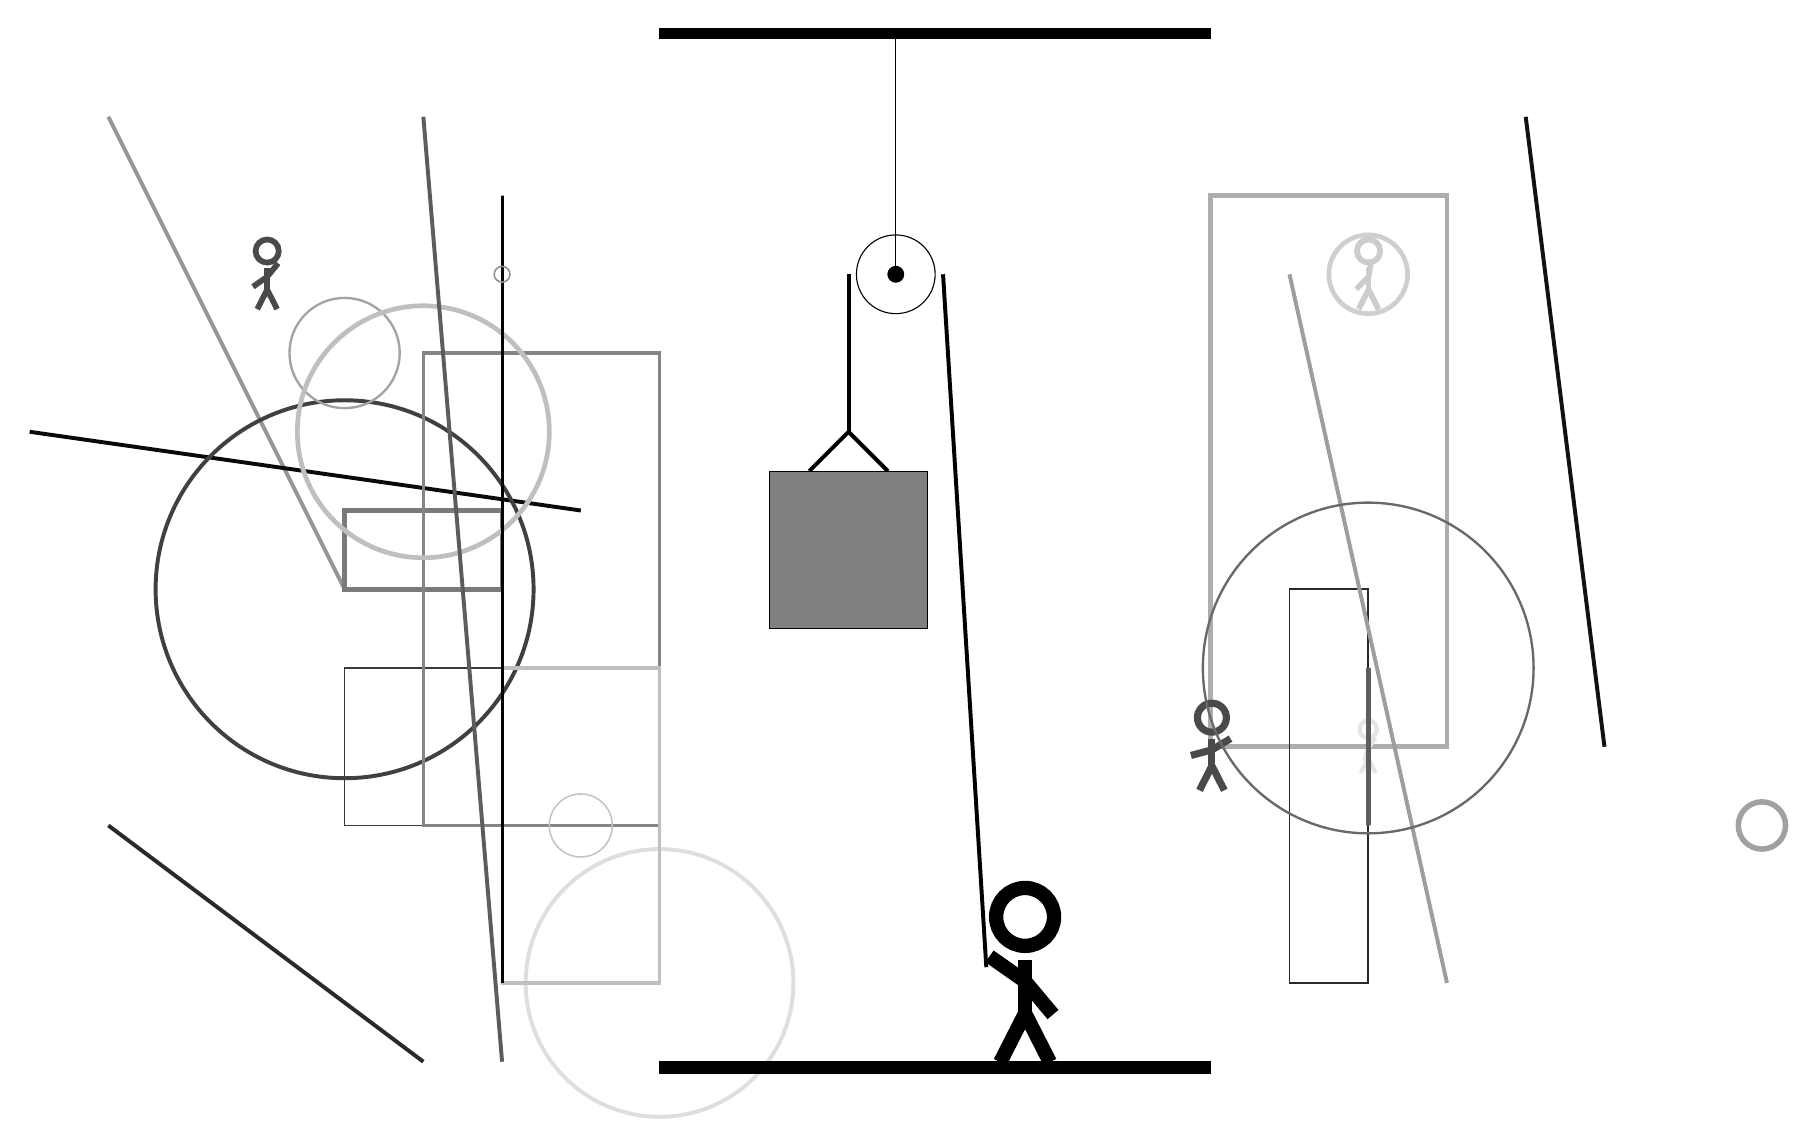
\begin{tikzpicture}
		%%%%% START %%%%%
		
		\draw[fill=black] (-2, 10) rectangle (5, 10.125);
		
		\draw (1, 7) circle (0.5);
		\draw[fill=black] (1, 7) circle (0.1);
		\draw (1, 10) -- (1, 7);
		
		\draw [line width=0.6mm, color=black!19](7, 7) circle (0.5);
		
		\draw[line width=0.2mm, color=black!77] (-2, 2) rectangle (-6, 0);
		\draw[line width=0.5mm, color=black!41](-6, 3) -- (-9, 9);
		\draw[line width=0.6mm, color=black!52] (-4, 4) rectangle (-6, 3);
		\draw[line width=0.6mm, color=black!32] (5, 1) rectangle (8, 8);
		\draw[line width=0.2mm, color=black!84] (7, -2) rectangle (6, 3);
		
		\node[line width=0.7mm, color=black!71] at (-7, 7) {\Strichmaxerl[4][35][51]};
		\draw[line width=0.5mm, color=black!96](-3, 4) -- (-10, 5);
		\draw [line width=0.7mm, color=black!37](12, 0) circle (0.3);
		\draw [line width=0.5mm, color=black!13](-2, -2) circle (1.7);
		
		\draw [line width=0.5mm, color=black!75](-6, 3) circle (2.4);
		\node[line width=0.7mm, color=black!10] at (7, 1) {\Strichmaxerl[3][72][56]};
		\draw[line width=0.4mm, color=black!48] (-2, 0) rectangle (-5, 6);
		
		\draw [line width=0.3mm, color=black!36](-6, 6) circle (0.7);
		\draw[line width=0.5mm, color=black!93](10, 1) -- (9, 9);
		\draw[line width=0.4mm, color=black!25] (-4, 2) rectangle (-2, -2);
		\draw [line width=0.6mm, color=black!25](-5, 5) circle (1.6);
		
		\node[line width=0.5mm, color=black!20] at (7, 7) {\Strichmaxerl[4][45][81]};
		\draw[line width=0.5mm, color=black!84](-5, -3) -- (-9, 0);
		\node[line width=0.3mm, color=black!71] at (5, 1) {\Strichmaxerl[5][15][31]};
		\draw[line width=0.6mm, color=black!63] (7, 2) rectangle (7, 0);
		
		\draw[line width=0.5mm, color=black!64](-4, -3) -- (-5, 9);
		\draw [line width=0.2mm, color=black!23](-3, 0) circle (0.4);
		\draw[line width=0.4mm, color=black!99] (-4, 8) rectangle (-4, -2);
		\draw [line width=0.2mm, color=black!44](-4, 7) circle (0.1);
		
		\draw[line width=0.5mm, color=black!38](8, -2) -- (6, 7);
		\draw [line width=0.3mm, color=black!59](7, 2) circle (2.1);
		
		\draw[line width=0.5mm] (-0.1, 4.5) -- (0.4, 5.0) -- (0.9, 4.5);
		\draw[fill=black!50] (-0.6, 4.5) rectangle (1.4, 2.5);
		
		\draw[line width=0.5mm] (0.4, 7) -- (0.4, 5.0);
		\centerarc[line width=0.5mm](1, 7)(0:180:0.6);
		\draw[line width=0.5mm](1.6, 7) -- (2.15, -1.8);
		
		\node at (2.6, -1.9) {\Strichmaxerl[10][-35][-50]};
		
		\draw[fill=black] (-2, -3) rectangle (5, -3.15);
		
		%%%%% END %%%%%
	\end{tikzpicture}
\end{document}